\documentclass[a4paper]{article}
\usepackage[dutch]{babel}
\usepackage{mathtools}
\usepackage{graphicx}
\graphicspath{ {Afbeeldingen/}}
\title{Practicum Numerieke Wiskunde}
\author{Barbara Ameloot, Tobias Baert}
\date{Mei 2018}
\begin{document}
\maketitle
   \section*{Opdracht 1.1}
Het matrixproduct  $A=L_{E}\cdot U$ :
\\
\[
 \begin{bmatrix}
  a_{1,1} & a_{1,2} & \cdots & a_{1,n} \\
  a_{2,1} & a_{2,2} & \cdots & a_{2,n} \\
  \vdots  & \vdots  & \ddots & \vdots  \\
  a_{n,1} & a_{n,2} & \cdots & a_{n,n} 
 \end{bmatrix}
=
\begin{bmatrix}
 1 & 0 & \cdots & 0 \\
  l_{2,1} &1 & \cdots &0 \\
  \vdots  & \vdots  & \ddots & \vdots  \\
  l_{n,1} &l_{n,2} & \cdots & 1 
\end{bmatrix}
\cdot
\begin{bmatrix}
  u_{1,1} & u_{1,2} & \cdots & u_{1,n} \\
  0 & u_{2,2} & \cdots & u_{2,n} \\
  \vdots  & \vdots  & \ddots & \vdots  \\
 0 & 0 & \cdots & u_{n,n}
\end{bmatrix}
\]
\\
\begin{minipage}[c]{\textwidth}
%\begin{samepage} %elementen op zelfde pagina houden
Als we de elementen van dit matrixproduct elementgewijs uitschrijven krijgen we:
\begin{tabbing} %voor layout
\\$a_{1,1} = 1 \cdot u_{1,1}$\hspace{6.0cm} \= $\rightarrow  u_{1,1} = a_{1,1}$
\\$a_{1,2} = 1 \cdot u_{1,2}$ \> $\rightarrow  u_{1,2}= a_{1,2}$
\\$a_{1,3} = 1 \cdot u_{1,3}$ \> $\rightarrow  u_{1,3}= a_{1,3}$
\\ {...}
\\$a_{1,n} = 1 \cdot u_{1,n}$ \> $\rightarrow  u_{1,n}= a_{1,n}$
\\ {}
\\$a_{2,1} = l_{2,1} \cdot u_{1,1}$ \> $\rightarrow l_{2,1}$
\\$a_{2,2} = l_{2,1} \cdot u_{1,2} + 1 \cdot u_{2,2}$ \> $\rightarrow u_{2,2}$
\\$a_{2,3} = l_{2,1} \cdot u_{1,3} + 1 \cdot u_{2,3}$ \> $\rightarrow u_{2,3}$
\\{...}
\\$a_{2,n} = l_{2,1} \cdot u_{1,n} + 1 \cdot u_{2,n}$ \> $\rightarrow u_{2,n}$
\\{}
\\$a_{3,1} = l_{3,1} \cdot u_{1,1}$ \> $\rightarrow l_{3,1}$
\\$a_{3,2} = l_{3,1} \cdot u_{1,2} +  l_{3,2} \cdot u_{2,2}$ \> $\rightarrow l_{3,2}$
\\$a_{3,3} = l_{3,1} \cdot u_{1,3} +  l_{3,2} \cdot u_{2,3} + 1 \cdot u_{3,3}$ \> $\rightarrow u_{3,3}$
\\{...}
\\$a_{3,n} = l_{3,1} \cdot u_{1,n} +  l_{3,2} \cdot u_{2,n} + 1 \cdot u_{3,n}$ \> $\rightarrow u_{3,n}$
\\{}
\\$a_{4,1} = l_{4,1} \cdot u_{1,1}$ \> $\rightarrow l_{4,1}$
\\$a_{4,2} = l_{4,1} \cdot u_{1,2} +  l_{4,2} \cdot u_{2,2}$ \> $\rightarrow l_{4,2}$
\\$a_{4,3} = l_{4,1} \cdot u_{1,3} +  l_{4,2} \cdot u_{2,3} + l_{4,3} \cdot u_{3,3}$ \> $\rightarrow l_{4,3}$
\\$a_{4,4} = l_{4,1} \cdot u_{1,4} +  l_{4,2} \cdot u_{2,4} + l_{4,3} \cdot u_{3,4} + 1 \cdot u_{4,4}$ \> $\rightarrow u_{4,4}$
\\{...}
\\$a_{4,n} = l_{4,1} \cdot u_{1,n} +  l_{4,2} \cdot u_{2,n} + l_{4,3} \cdot u_{3,n} + 1 \cdot u_{4,n}$ \> $\rightarrow u_{4,n}$
\\{}
\end{tabbing}
\end{minipage}
\pagebreak
%Elementen berekenen
\begin{verse}
\begin{tabbing}
We kunnen de elementen $u_{i,j}$ en $ l_{i,j}$ van $U$ en $L_{E}$ als volgt berekenen:
\\Voor $i = j \Rightarrow$  \= 
\\ \>$u_{i,j} =  a_{i,j}$
\\ \>$l_{i,j} =  1$
\\{}
\\Voor $i < j \Rightarrow$
\\ \>$u_{i,j} =  a_{i,j}$
\\ \>$l_{i,j} =  0$
\\{}
\\Voor $i > j  \Rightarrow$ 
\\ \>$u_{i,j} =  0$
\\ \>$l_{i,j} =  a_{i,j}$
\end{tabbing}
\end{verse}
\section*{Opdracht 1.2}
Voor de matrix $U$:
\\Uit 1.1 weten we dat als $u_{i,j}$ onder de hoofddiagonaal valt, $u_{i,j} = 0$.
\\In het andere geval (element ligt op de hoofddiagonaal of erboven) is $u_{i,j} = a_{i,j}$.
\\Omdat $A$ een tridiagonale matrix is zijn alle elementen van $A$ boven de superdiagonaal $0$.
\\Alle elementen van $U$ boven de superdiagonaal zijn dus ook 0.
\\$U$ is dus een tridiagonale matrix.
\\{}
\\Voor de matrix $L$:
\\Uit 1.1 weten we dat als $l_{i,j}$ boven de hoofddiagonaal valt, $l_{i,j} = 0$.
\\Als $l_{i,j}$ op de hoofddiagonaal ligt, is $l_{i,j} = 1$.
\\Als $l_{i,j}$ onder de hoofddiagonaal ligt is $l_{i,j} = a_{i,j}$.
\\Omdat $A$ een tridiagonale matrix is zijn alle elementen van $A$ onder de subdiagonaal $0$.
\\Alle elementen van $L$ onder de subdiagonaal zijn dus ook 0.
\\$L$ is dus een tridiagonale matrix.
\section*{Opdracht 1.3.1}
Aantal elementaire bewerkingen:
\\$(n-1) \cdot 6V + (n-1) \cdot 3O$
\\Met $V$: vermenigvuldiging/deling en $O$: optelling/aftrekking
\section*{Opdracht 1.3.2}
Er wordt reeds in het begin van het algoritme een nul-element gevormd op de hoofddiagonaal van U. In een volgende stap wordt door dit element gedeeld.
\section*{Opdracht 1.3.3}
TODO
\section*{Opdracht 2.4}
Plot:
\\{}
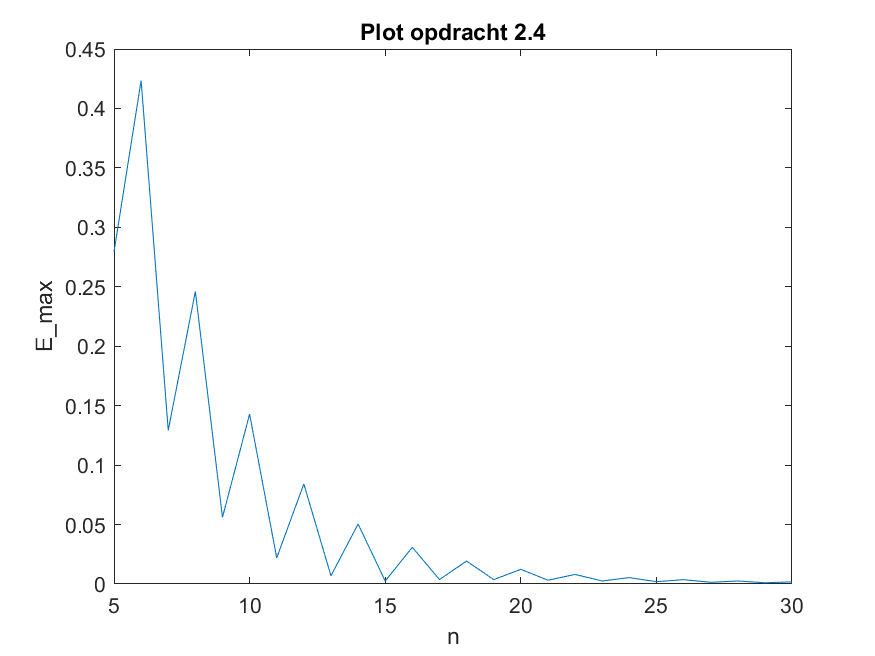
\includegraphics[scale = 0.8]{plot2_4}
\section*{Opdracht 2.5}
Plot:
\\{}
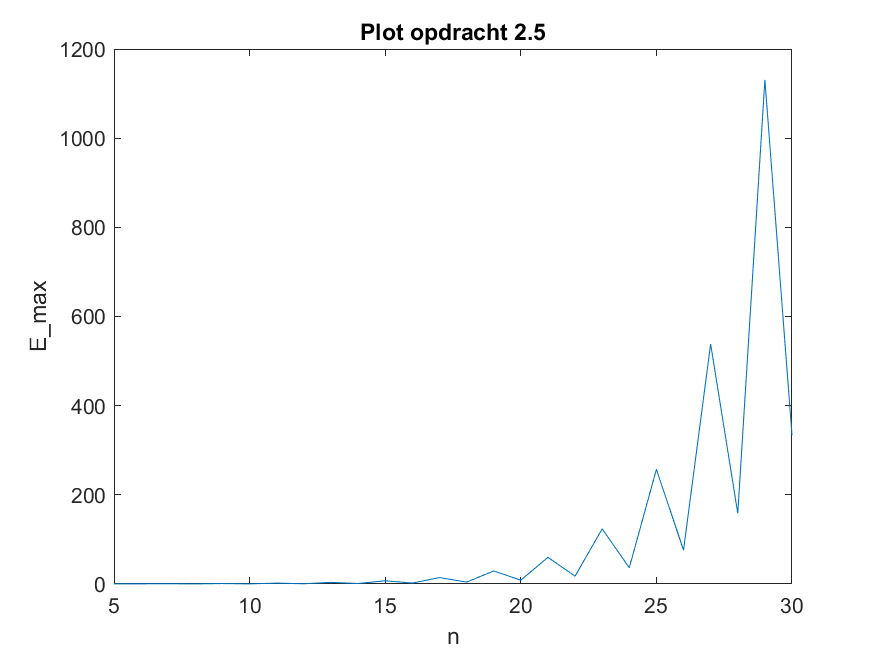
\includegraphics[scale = 0.8]{plot2_5}
\section*{Opdracht 2.6}
We kunnen meteen inzien dat methode uit opdracht 2.4 een betere benadering oplevert dan de  methode uit opdracht 2.5 zolang het aantal knooppunten groot genoeg is. Het belangrijkste verschil tussen de twee methodes is het gebrek aan convergentie bij de methode uit opdracht 2.5. Dat is een gevolg van het verschijnsel van Runge. Interpolaties met equidistante knooppunten van bepaalde functies, waaronder de Runge-functie, convergeren niet. De benadering begint sterk te oscilleren aan de randen van het interpolatieinterval, met een grote maximale interpolatie fout als gevolg.
\end{document}

